\documentclass[12pt]{article}

\usepackage{mathtools}
\usepackage{amssymb}
\usepackage{atbegshi}% http://ctan.org/pkg/atbegshi
\usepackage{graphicx}
\usepackage{physics}
\AtBeginDocument{\AtBeginShipoutNext{\AtBeginShipoutDiscard}}

\usepackage{fontspec}
\defaultfontfeatures{Mapping=tex-text,Scale=MatchLowercase}
\setmonofont{Consolas}


\begin{document}

\title{Tarea 21\\
	\large Elementos de ciencias de la computación}

\author{Tulio Muñoz Magaña}
\today
\maketitle

\textbf{Inciso a)} El programa \texttt{print\_pointers.c} está hecho para enseñar las diferentes formas de mostrar en pantalla una dirección de memoria. Crea dos variables enteras y muestra sus direcciones en 3 formatos, \texttt{\%p}, \texttt{\%x} y \texttt{\%u}.\\
Al desplegar la dirección en \texttt{printf} con \texttt{\%p}, de despliega el apuntador como apuntador de tipo \texttt{void*}, se muestra la dirección completa en hexadecimal, por lo que se muestran 16 dígitos en una computadora de 64 bits o 8 en una de 32, ya que en hexadecimal cada dígito representa 4 bits, en este formato se despliegan en mayúsculas los dígitos \texttt{A}, \texttt{B}, \texttt{C}, \texttt{D}, \texttt{E} y \texttt{F}. Al desplegar el apuntador con \texttt{\%x} se remueven los ceros a la izquierda de la dirección en hexadecimal, además de que se despliegan en minúsculas los dígitos \texttt{a}, \texttt{b}, \texttt{c}, \texttt{d}, \texttt{e} y \texttt{f}. Al mostrar un apuntador con el formato \texttt{\%u}, se interpreta como \texttt{unsigned int}, por lo que se despliega la dirección en decimal.\\\\

\textbf{Inciso b)} El código se encuentra en el proyecto "Tarea 21".\\

Vemos en las capturas que los pasos que realizan los apuntadores son de diferentes distancias para cada tipo de dato, ya que cada tipo de dato ocupa una cantidad diferente de bytes (las direcciones están desplegadas en hexadecimal).\\

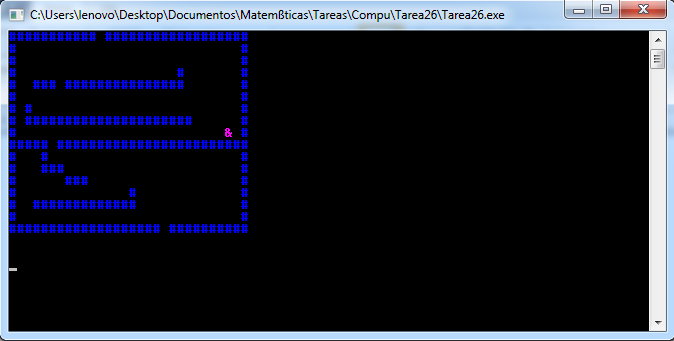
\includegraphics[width = \textwidth]{captura1}




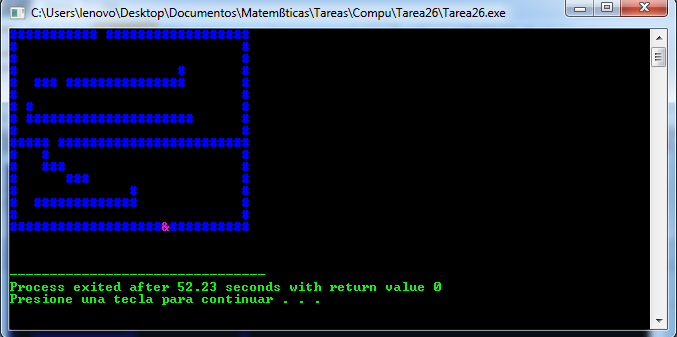
\includegraphics[width = \textwidth]{captura2}\\

A continuación se muestran los pasos que dan los apuntadores para cada tipo de dato (en bytes):\\

{\setlength\parindent{0pt}

char $\leftrightarrow$ 1\\
int $\leftrightarrow$ 4\\
unsigned int $\leftrightarrow$ 4\\
float $\leftrightarrow$ 4\\
double $\leftrightarrow$ 8\\
long double $\leftrightarrow$ 16\\


}






















\end{document}